\documentclass[10pt, a4paper, oneside, fontset=none]{ctexart}
%调用宏包
\usepackage{amsmath, amsthm, amssymb, graphicx, wrapfig, mathrsfs, upgreek}
\usepackage[bookmarks=true, colorlinks, citecolor=blue, linkcolor=black]{hyperref}
\usepackage{color, framed, geometry, tcolorbox, multirow, booktabs}
\tcbuselibrary{breakable}%box跨页
\tcbuselibrary{skins}%box跨页不留边
%\usepackage{CJKpunct}
\usepackage{makecell, booktabs, longtable}
\usepackage[font=sf, labelfont+=bf]{caption}
\usepackage[font={small, sf}]{subfig}
\usepackage{multicol}
\usepackage{arydshln, nicematrix}%矩阵
\usepackage{extarrows}
\usepackage[american,]{circuitikz}
\usepackage{xpatch}
\usepackage{rotating}%旋转
\usepackage{physics}
\usepackage{esint}
\usepackage{enumitem}
\usepackage{dashrule}% 虚线分割线
\usepackage[text=\includegraphics{C:/Users/16870/.vscode/LaTeX_Application/tex/THUEE23-23Autumn/图标简稿.png},angle=0]{draftwatermark}%水印
%\usepackage{tikz}
%-------------基本字体设置--------------
\catcode`\,=\active
\def ,{\textup{,}\hskip0.5em }
%\usepackage[math-style=ISO, bold-style=ISO]{unicode-math}
%\setmainfont{EB Garamond}%You should have installed the font
%\setmathfont{Garamond-Math.otf}[StylisticSet={7,9}]
%\setmathsfont(Digits,Latin){Garamond MT Pro}
%\setmathfont{latinmodern-math.otf}
%\setmathfont{方正书宋_GBK}[range="002C]
\setmonofont{Iosevka}
\setCJKmainfont{FZXSSK.TTF}[BoldFont={SourceHanSerifCN-Bold.otf}, ItalicFont={FZXKTK.TTF}, BoldItalicFont={汉仪颜楷W.ttf}]
\setCJKsansfont{汉仪文黑-45W.ttf}[BoldFont={汉仪文黑-75W.ttf}, ItalicFont={FZYanZQKSJF.TTF}]
\setCJKmonofont{LXGWNeoXiHei.ttf}
%附加字体设置
\newCJKfontfamily{\kaico}{可口可乐在乎体 楷体Coca-ColaCareFontKaiTi.TTF}
\newCJKfontfamily{\kai}{FZXKTK.TTF}[BoldFont={汉仪颜楷W.ttf}, ItalicFont={方正清刻本悦宋 简繁.TTF}, BoldItalicFont={FZYanZQKSJF.TTF}]
\newCJKfontfamily{\yan}{方正清刻本悦宋 简繁.TTF}[ItalicFont={FZYanZQKSJF.TTF}]
\newCJKfontfamily{\xiu}{方正宋刻本秀楷_GBK.TTF}[ItalicFont={方正宋刻本秀楷_GBK.TTF}, BoldFont={FZYanZQKSJF.TTF}]
\newCJKfontfamily{\run}{汉仪润圆-45W.ttf}[BoldFont={汉仪润圆-75W.ttf}, ItalicFont={汉仪润圆-45W.ttf}]
\newCJKfontfamily{\wen}{汉仪文黑-45W.ttf}[BoldFont={汉仪文黑-75W.ttf}, ItalicFont={hk4e_zh-cn.ttf}]
%文档格式
\geometry{left=2.24cm, right=2.24cm, top=3.18cm, bottom=3.18cm}
\setcounter{tocdepth}{3}
\setcounter{secnumdepth}{4}
\linespread{1.4}
\numberwithin{equation}{subsection}
\renewcommand{\theparagraph}{\Alph{paragraph})}
\newcommand{\Section}[1]{ \refstepcounter{section} \section*{*\thesection\texorpdfstring{\quad}{}#1} \addcontentsline{toc}{section}{\makebox[0pt][r]{*}\thesection\texorpdfstring{\quad}{}#1} }
\newcommand{\Subsection}[1]{ \refstepcounter{subsection} \subsection*{*\thesubsection\texorpdfstring{\quad}{}#1} \addcontentsline{toc}{subsection}{\makebox[0pt][r]{*}\thesubsection\texorpdfstring{\quad}{}#1} }
\newcommand{\Subsubsection}[1]{ \refstepcounter{subsubsection} \subsubsection*{*\thesubsubsection\texorpdfstring{\quad}{}#1} \addcontentsline{toc}{subsubsection}{\makebox[0pt][r]{*}\thesubsubsection\texorpdfstring{\quad}{}#1} }
\setlist[itemize]{leftmargin=3em, labelsep=0.25em, itemindent=0em, itemsep=0pt, parsep=0pt, topsep=3pt, partopsep=0pt}
\setlength{\lineskip}{5pt}
\setlength{\lineskiplimit}{5pt}
\setlength{\belowcaptionskip}{-1em}
\setlength{\abovecaptionskip}{0.5em}
\setlength{\columnsep}{1cm} % 分栏间距
\setlength{\columnseprule}{.4pt} % 栏分割线粗
\setlength{\abovecaptionskip}{0.2em}
\setlength{\belowcaptionskip}{-0.5em}
\def\columnseprulecolor{\color{white!50!black}}

\captionsetup[subfigure]{captionskip=0.5em, nearskip=-0.5em}
\ctikzset{monopoles/vcc/arrow={Stealth[width=4pt, length=6pt]}}
\ctikzset{monopoles/vee/arrow={Stealth[width=4pt, length=6pt]}}
\ctikzset{bipoles/length=1cm}
%\punctstyle{kaiming}
%定理环境
\theoremstyle{plain}
\newtheorem{theorem}{  定理}[subsection]
\newtheorem{definition}{  定义}[subsection]
\newtheorem{law}[theorem]{  定律}
\newtheorem{lemma}[theorem]{  引理}
\newtheorem{corollary}[theorem]{  推论}
\newtheorem{proposition}[theorem]{  命题}

\theoremstyle{definition}
\newtheorem{Example}{  实例}
\newtheorem{examplein}[theorem]{\run 例题}
\newtheorem{circum}[theorem]{情形}

\newcommand{\exampleparameter}{0}
\newenvironment{example}[1][0]{% 0/1: no space; 2/3: 5pt space
	\renewcommand{\exampleparameter}{#1}
	\ifnum \exampleparameter>1
		\vspace{10pt}
	\fi
	\hrule
	\vspace{3pt}
	\noindent\hdashrule{\linewidth}{0.5pt}{2pt}
	\vspace{-2em}
	\begin{examplein}
}{% 0/2: -0.5pt space; 1/3: 5pt space
	\end{examplein}
	\vspace{-1em}
	\noindent\hdashrule{\linewidth}{0.5pt}{2pt}\vspace{3pt}
	\hrule
	\ifnum 1=\exampleparameter
		\vspace{10pt}
	\else
		\ifnum 3=\exampleparameter
			\vspace{10pt}
		\else
			\vspace{-0.5pt}
		\fi
	\fi
}

\newenvironment{proofs}[1][\proofname]{\begin{pf}[breakable, enhanced jigsaw]\begin{proof}[\small\yan{#1}]\small\kai}{\end{proof}\end{pf}}
\newenvironment{solution}[1][解]{\begin{proofs}[\small\textit{\yan #1}]\small\renewcommand{\qedsymbol}{$\circledS$}}{\end{proofs}}
\renewcommand{\proofname}{\yan{证明}}

\renewenvironment{abstract}{\begin{prenote}{提要}
	\lineskiplimit=5pt
	\lineskip=4pt
	\abovedisplayskip=1pt
	\belowdisplayskip=0pt
	\begin{description}[align=left, itemindent=1em, labelsep=1em, leftmargin=0pt]
}{\end{description}\end{prenote}}

\renewenvironment{cases}[1][l]{\left\{\begin{NiceArray}{#1}}{\end{NiceArray}\right.}

%颜色命名
\definecolor{meihong}{rgb}{0.85,0.2,0.47}
\definecolor{bali}{rgb}{0.2,0.6,0.78}
\definecolor{qinglv}{rgb}{0,0.35,0.32}
%box环境
\newtcolorbox{pr}[2][]{colback=black!5!white,colframe=white!75!black,fonttitle=\sffamily\wen\bfseries,title=#2,#1}
\newtcolorbox[use counter=definition,number within=subsection]{defi}[2][]{colback=bali!5!white,colframe=bali!75!black,fonttitle=\sffamily\wen\bfseries,fontlower=\kai\small,title=定义~\thetcbcounter. #2,#1}
\newtcolorbox[auto counter,number within=section]{compl}[2][]{colback=bali!5!white,colframe=bali!65!black,fonttitle=\sffamily\wen\bfseries,label=#2,title=电路部件~\thetcbcounter. #2,#1, fontupper=\kai, fontlower=\kai}
\newtcolorbox[use counter=theorem,number within=subsection]{theo}[2][]{colback=meihong!5!white,colframe=meihong!75!black,fonttitle=\sffamily\wen\bfseries,fontupper=\run,fontlower=\run\small,title=结论~\thetcbcounter. #2,#1}
\newtcolorbox[use counter=definition,number within=subsection]{defil}[2][]{colback=bali!5!white,colframe=bali!75!black,fonttitle=\sffamily\wen\bfseries,fontlower=\kai\small,label=#2,title=定义~\thetcbcounter. #2,#1}
\newtcolorbox[use counter=theorem,number within=subsection]{theol}[2][]{colback=meihong!5!white,colframe=meihong!75!black,fonttitle=\sffamily\wen\bfseries,fontupper=\run,fontlower=\run\small,label=#2,title=结论~\thetcbcounter. #2,#1}
\newtcolorbox[auto counter,number within=section]{note}[2][]{colback=qinglv!5!white,colframe=qinglv!75!black,breakable, enhanced jigsaw,fonttitle=\sffamily\wen\bfseries,title=注~\thetcbcounter. #2,#1}
\newtcolorbox{prenote}[2][]{colback=gray!5!white,colframe=gray!50!black,breakable, enhanced jigsaw, fonttitle=\sffamily\wen\bfseries,fontupper=\small\kai,title=#2,#1}
\newtcolorbox{pf}[1][]{colback=black!5!white,colframe=white!75!black, fontupper=\small\kai, breakable, enhanced jigsaw, #1}
\newtcolorbox[auto counter]{eg}[2][]{colback=black!5!white,colframe=white!75!black, breakable, enhanced jigsaw, fontupper=\small, breakable, enhanced jigsaw, fonttitle=\sffamily\wen\bfseries, title=实例~\thetcbcounter\quad#2, #1}
%\newcommand{\mybox}[1]{\tikz[baseline=(MeNode.base)]{\node[rounded corners, fill=gray!20](MeNode){#1};}}

\newcommand{\hang}[1][1]{\hangafter 1 \hangindent #1em \noindent}
\newcommand{\com}[1][0.3]{,\uskip0.8em\uskip-#1em}
\newcommand{\page}[1]{\ufill P$_\text{#1}$}
\newcommand{\colors}[1]{\color{#1!75!black}}
\newcommand{\paratitle}[1]{\hang \textbf{\wen #1}\uskip1em}
\newcommand{\tboqi}[1]{\textbf{\color{qinglv!75!black}#1}}
\newcommand{\mboqi}[1]{\boldsymbol{\color{qinglv!75!black}#1}}
\newcommand{\tboba}[1]{\textbf{\color{bali!75!black}#1}}
\newcommand{\mboba}[1]{\boldsymbol{\color{bali!75!black}#1}}
\newcommand{\tbome}[1]{\textbf{\run\color{meihong!75!black}#1}}
\newcommand{\mbome}[1]{\run\boldsymbol{\color{meihong!75!black}#1}}
\newcommand{\den}[2][]{\begin{defi}{#1}
	\kai #2\end{defi}}
\newcommand{\din}[2][]{\begin{theo}{#1}
	\run #2\end{theo}}
\newcommand{\de}[2][]{\begin{defil}{#1}
	\kai #2\end{defil}}
\newcommand{\di}[2][]{\begin{theol}{#1}
	\run #2\end{theol}}
\newcommand{\dep}[3][]{\begin{defi}{#1\page{#2}}
	\kai #3\end{defi}}
\newcommand{\dip}[3][]{\begin{theo}{#1\page{#2}}
	\run #3\end{theo}}
\newcommand{\zhu}[2][]{\begin{note}{#1}
	\xiu #2\end{note}}
\newcommand{\bu}[3][]{\begin{compl}{#1}	\paratitle{记号}#2 \tcblower\paratitle{特性}#3\end{compl}}
\newcommand{\btheo}{\begin{theo}}
\newcommand{\etheo}{\end{theo}}	
\newcommand{\trans}[2][注]{\marginpar{
		\begin{prenote}{#1}
			\raggedright
			#2
		\end{prenote}
	}}
\newcommand{\tranS}[3][-1]{\marginnote{
		\begin{prenote}{#2}
			\raggedright
			#3
		\end{prenote}
	}[#1\baselineskip]}
\newcommand{\cbox}[1]{
	$\vcenter{\ubox{\begin{circuitikz}
		#1
	\end{circuitikz}}}$
}
\newcommand{\shbox}[1]{\cbox{\draw (0,0) to[#1] (1.5,0);}(\texttt{#1})}
%定义算符
\newcommand{\rref}{\mathrm{rref}}
\newcommand{\C}{\mathbb{C}}
\renewcommand{\i}{\mathrm{i}}
\newcommand{\neiji}[4]{\boldsymbol{#1}_{#3}^\mathrm{T}\boldsymbol{#2}_{#4}}
\def\upint{\mathchoice%
	{\mkern13mu\overline{\vphantom{\intop}\mkern7mu}\mkern-20mu}%
	{\mkern7mu\overline{\vphantom{\intop}\mkern7mu}\mkern-14mu}%
	{\mkern7mu\overline{\vphantom{\intop}\mkern7mu}\mkern-14mu}%
	{\mkern7mu\overline{\vphantom{\intop}\mkern7mu}\mkern-14mu}%
	\int}
\def\lowint{\mkern3mu\underline{\vphantom{\intop}\mkern7mu}\mkern-10mu\int}
\renewcommand{\a}[1]{\left\langle #1 \right\rangle}
\newcommand{\V}{\vee}
\newcommand{\A}{\wedge}
\newcommand{\Lr}{\Longleftrightarrow}
\newcommand{\LLr}[2][]{\xLongleftrightarrow[#1]{#2}}
\newcommand{\dbar}{\mathop{}\!\;\bar{}\hspace{-0.3em}\mathrm{d}}
\newcommand{\dif}{\mathop{}\!\mathrm{d}}
\newcommand{\Dif}{\mathop{}\!\Delta}
\newcommand{\e}{\mathrm{e}}
\newcommand{\upi}{\uppi}
\newcommand{\R}{\mathbb{R}}
\newcommand{\bF}{\mathbb{F}}
\newcommand{\dint}{\displaystyle\int}
\renewcommand{\cfrac}[2]{\genfrac{}{}{}{0}{\raisebox{0.6em}{$#1$}}{\raisebox{-0.8em}{$#2$}}}
\newcommand{\cufrac}[2]{\genfrac{}{}{}{0}{\raisebox{0.6em}{$#1$}}{#2}}
\newcommand{\cdfrac}[2]{\genfrac{}{}{}{0}{#1}{\raisebox{-0.8em}{$#2$}}}
\renewcommand{\v}[1]{{\va*{#1}}}
%\renewcommand{\v}[1]{{\overrightarrow{#1}}}
\newcommand{\vr}{\v{r}}
\newcommand{\vv}{\v{v}}
\newcommand{\voa}{\v{a}}
\newcommand{\ux}{\vu*{x}}
\newcommand{\uy}{\vu*{y}}
\newcommand{\uz}{\vu*{z}}
\newcommand{\ur}{\vu*{r}}
\newcommand{\uq}{\vu*{\theta}}
\newcommand{\dt}[1][]{\dfrac{\dif #1}{\dif t}}
%标题、作者、日期
\title
{
	\textbf{大学物理A(2)}{\kai 知识与方法}
}
\author{\zihao{5} T$^\text{T}$T}
\date{\zihao{5} \kai \today}
%----------------------------------------------------------
\begin{document}

\maketitle
\begin{multicols}{2}
	\begin{flushleft}
		\tableofcontents
	\end{flushleft}
\end{multicols}

\setcounter{section}{4}
\newpage
%----------------------------------------------------------
\section{热学}

\setcounter{subsection}{-1}
\subsection{绪言}

\subsubsection{热学基本概念}

\de[热力学系统]{
	\tboba{大量}微观粒子(分子、原子)构成的\tboba{体积有限}的物体。
}

热力学系统分为:
\begin{itemize}
	\item \tboba{孤立系统}:与外界无能量、物质交换;
	\item \tboba{封闭系统}:与外界无物质交换,有能量交换;
	\subitem \tboba{绝热系统}:与外界只有力学相互作用,即除有功交换之外与外界无能量交换的封闭系统。
	\item \tboba{开放系统}:与外界有能量、物质交换。
\end{itemize}

热学的研究方法:
\begin{itemize}
	\item \tboba{热力学}:从宏观基本实验规律出发,研究热力学系统的性质;
	\item \tboba{统计物理}:从微观的模型、假设出发,研究热力学系统的性质。
\end{itemize}

\de[平衡态]{
	热力学系统内部没有\tboba{宏观}的粒子和能量流动状态,系统各种\tboba{宏观}性质不随时间变化。
}

\di[平衡条件]{
	与外界有相互作用的系统要保持平衡态,应满足\tbome{平衡条件},如:
	\begin{itemize}
		\item \tbome{力学平衡条件}:系统与外界有力学相互作用,则平衡时系统内外压强相等;
		\item \tbome{热平衡条件}:	系统与外界有热量交换,则平衡时系统内外温度相等;
		\item \tbome{相平衡条件}:	系统与外界处于不同相,则平衡时系统内外相同;
		\item \tbome{化学平衡条件}:系统与外界是浓度不同的两种物质,则平衡时系统内外浓度相等。
	\end{itemize}
}

\zhu[区分热力学系统的平衡态和稳定态]{
	
}

\de[宏观量]{
	表征热力学系统宏观性质的物理量,如温度、压强、体积、熵等。
	\begin{itemize}
		\item \tboba{广延量}:有累加性质,\( \lim\limits_{N \to \infty} \dfrac{Ex}{N} = \mathrm{Constant}\),如体积、质量、熵等;
		\item \tboba{强度量}:无累加性质,\( \lim\limits_{N \to \infty} In = \mathrm{Constant}\),如温度、压强、密度等。
	\end{itemize}
}

\begin{definition}
	\textbf{物态参量}是指描述热力学系统平衡态的宏观量。一组物态参量可以唯一确定系统的平衡态。
\end{definition}
\begin{definition}
	处于平衡态的热力学系统的物态参量之间的关系称为\textbf{物态方程}。
\end{definition}

\begin{eg}{理想气体物态方程}
	由理想气体构成的热力学系统,其物态方程为\( pV = \dfrac{m}{M}RT \),其中\( p \)为气体压强,\( V \)为气体体积,\( m \)为气体质量,\( M \)为气体摩尔质量,\( R \)为气体常数,\( T \)为气体温度。

	理想气体物态方程还可以表示为\( p = nkT \),其中\( n \)为气体分子的数密度,\( k = \dfrac{R}{N_\mathrm{A}} \approx  1.38 \cp 10^{-23} \mathrm{\,J/mol} \)为玻尔兹曼常数。
\end{eg}

\subsection{气体动理论}

\subsubsection{温度}

\begin{definition}
	\textbf{热平衡态}是指两个物体之间长时间热接触所达到的没有热量交换的共同平衡态。
\end{definition}

\begin{law}
	\textup{\textbf{热力学第零定律}}\quad 如果两个物体分别与第三个物体热平衡,那么这两个物体之间也处于热平衡。
\end{law}

\begin{definition}
	\textbf{温度}是描述物体热平衡状态的物态参量,是处于同一热平衡态下的热力学系统所具有的共同的宏观性质。
\end{definition}

一切处于同一热平衡态的系统具有相同温度。
温度取决于系统内微观粒子的热运动状态。

\begin{definition}
	\textbf{温标}是衡量温度数值的规则。常见常用的温标有:
	\begin{itemize}
		\item \textbf{理想气体温标}:以理想气体的等温过程为基础,将气体的温度定义为正比于气体的压强 \(p\) 与体积 \(V\) 的乘积的量,并规定水的三相点温度为\(T_3 = 273.16\mathrm{\,K}\)。
		\item \textbf{热力学温标}:不依赖测温物质及其测温属性的温标,在理想气体温标有效范围内与理想气体温标一致,用 \(T\) 表示。
		\item \textbf{摄氏温标}:用 \(t\) 表示,与热力学温标满足 \(t = T - T_0\),其中 \(T_0 = 273.15\mathrm{\,K}\)。
		\item \textbf{华氏温标}:用 \(t_F\) 表示,与摄氏温标满足 \(t_F = \dfrac{9}{5}t + 32\)。
	\end{itemize}
\end{definition}

\begin{lemma}
	\textup{\textbf{大量分子处于平衡态时的统计假设}}\quad 大量分子处于平衡态时:

	(1)无外场时,分子在各处出现的概率相同:\(n = \dfrac{\dif N }{\dif V } = \dfrac{N }{V } = \mathrm{Constant}\)

	(2)由于碰撞,分子可以有各种不同的速度,且速度取向各方向等概率:\(\overline{\vv_x} = \overline{\vv_y} = \overline{\vv_z} = \v{0},\overline{\vv_x^2} = \overline{\vv_y^2} = \overline{\vv_z^2} = \dfrac{1}{3}\overline{\vv^2}\)
\end{lemma}

\di[理想气体压强公式]{
	平衡态下理想气体的压强公式为
	\begin{equation}
		p = \dfrac{2}{3}n\overline{\varepsilon}_t
	\end{equation}
	\tcblower
	\hang[3]\textbf{其中\quad}\( n \)——气体分子的数密度;\\
	\( \overline{\varepsilon}_t \)——气体分子的平均平动动能。 
}

由此与理想气体状态方程\(p=nkT\),可得理想气体分子的平均平动动能为\(\overline{\varepsilon}_t = \dfrac{3}{2}kT\),即 \(T\) 与 \(\overline{\varepsilon}_t\) 单值对应。\tbome{温度是大量分子热运动平均平动动能的量度}。

由平均平动动能\(\overline{\varepsilon}_t = \dfrac{1}{2}m\overline{\vv^2}\)和\(\overline{\varepsilon}_t = \dfrac{3}{2}kT\),得
\begin{equation}
	\overline{\vv^2} = \dfrac{3kT}{m} = \dfrac{3RT}{M} \propto T
	\quad \Rightarrow \quad \sqrt{\overline{\vv^2}} \propto \sqrt{T}
\end{equation}

\subsubsection{内能}

\begin{definition}
	气体分子\textbf{自由度}是指决定分子空间位置的独立坐标数目,用 \(i\) 表示,其可分为:
	\begin{itemize}
		\item \textbf{平动自由度}:分子在三个坐标轴上的运动自由度,用 \(t\) 表示;
		\item \textbf{转动自由度}:分子绕三个坐标轴的转动自由度,用 \(r\) 表示;
		\item \textbf{振动自由度}:分子内部原子之间的振动自由度,用 \(v\) 表示。
	\end{itemize}
\end{definition}

不同的分子结构有不同的自由度数目,如:
\begin{itemize}
	\item \textbf{单原子分子}:只有平动自由度,自由度 \(i = t = 3\);
	\item \textbf{双原子分子}:除平动自由度 \(t=3\) 外,还有轴取向的转动自由度 \(r=2\) 和轴向上的振动自由度	\(v=1\),总的自由度 \(i = t + r + v = 6\);
	\item \textbf{多原子分子}:用 \(N\) 表示单个分子中的原子数,则质心平动自由度 \(t=3\) ,刚体定点转动的转动自由度 \(r=3\) ,轴向上的振动自由度 \(v=3N-6\),总的自由度 \(i = 3N\)。
\end{itemize}

\di[能量均分定理]{
	在温度为 \(T\) 的热平衡状态下,分子热运动的每一个自由度所对应的平均动能都等于\(\dfrac{1}{2}kT\)。
}

更普遍地说,分子能量中每具有一个平方项,就对应一个\(\dfrac{1}{2}kT\)的平均能量。因此,对自由度 \(i = t + r + v \) 的非刚性分子,振动动能和振动势能都是平方项,其平均能量为
\begin{equation}
	\overline{\varepsilon} = \overline{\varepsilon}_t + \overline{\varepsilon}_r + \overline{\varepsilon}_v = (t + r + 2v) \dfrac{1}{2}kT
\end{equation}
通常情况下(\(T<10^3\mathrm{\,K }\)),分子的振动能量远小于平动和转动能量,可近似认为分子是刚性分子,只有平动和转动两种自由度,\(\overline{\varepsilon} = \dfrac{t + r }{2 }kT\)。

\de[内能]{
	系统内部各种形式能量的总和称为\tboba{内能},记作\(E\)。
	\begin{itemize}
		\item 在分子内部,内能包括分子的平动、转动、振动等能量,\(\overline{\varepsilon} = \overline{\varepsilon}_\mathrm{k } + \overline{\varepsilon}_\mathrm{p} = \dfrac{t+r+2v}{2}kT\);
		\item 在分子之间,内能包括分子间的相互作用势能 \(\varepsilon_{\mathrm{p}ij}\)。
	\end{itemize}
	总的内能 \(E = N\overline{\varepsilon} + \sum\limits_i \sum\limits_{j<i} \varepsilon_{\mathrm{p}ij} = E(T,V)\),它是系统温度和体积的函数。
}

\subsubsection{分子的速率和能量分布}

\de[速率分布函数]{
	设 \(\dif N_v \) 为速率在 \(v\) 到 \(v + \dif v \) 之间的分子数,\(\dif N \) 为总分子数,则应有 \(\dif N_v \propto N \dif v \) , 即 \(\dfrac{\dif N_v }{N } \propto \dif v \)。而 \(\dfrac{\dif N_v }{N }\) 是速率 \(v\) 附近 \(\dif v\) 区间内的分子数占总分子数的比例,应与 \(v\) 的大小有关,可令 \(\dfrac{\dif N_v }{N } = f(v) \dif v\),其中 \(f(v)\) 就称为\tboba{速率分布函数}。
}

由定义式
\begin{equation}
	f(v) = \dfrac{\dif N_v }{N \dif v }
\end{equation}
可以看出 \(f(v)\) 的意义,即速率 \(v\) 附近 \(\dif v\) 区间内的分子数占总分子数的比例,或一个分子处于速率 \(v\) 附近 \(\dif v\) 区间内的概率。于是我们有
\[
	\int_0^\infty f(v) \dif v = \int_{v=0}^\infty \dfrac{\dif N_v}{N} = 1
\]
这称为速率分布函数的\textbf{归一化条件}。

\paragraph{Maxwell 速率分布函数}
 
\di[Maxwell 速率分布函数]{
	无外场作用下,分子速率分布函数为
	\begin{equation}
		f(v) = 4\pi \left( \dfrac{m}{2\pi kT} \right)^{3/2} \e^{-{mv^2}/{2kT}} v^2
	\end{equation}
	\tcblower
	\hang[3]\textbf{其中\quad}\( m \)——分子质量;\\
	\( k \)——玻尔兹曼常数;\\
	\( T \)——系统温度。
}

\begin{definition}
	由 Maxwell 速率分布函数,可得分子的几种\tboba{统计速率}:
	\begin{itemize}
		\item \tboba{最概然(可几)速率}:速率分布函数的极大值对应的速率,记作\( v_\mathrm{p} \)。
		\begin{equation}
			v_\mathrm{p} \xlongequal{\left.\frac{\dif f(v)}{\dif v}\right|_{v=v_\mathrm{p}} = 0} \sqrt{\dfrac{2kT}{m}} = \sqrt{\dfrac{2RT}{M}} \propto \sqrt{T}
		\end{equation}
		\item \tboba{平均速率}:速率分布函数的平均值,记作\( \overline{v} \)。
		\begin{equation}
			\overline{v} = \dfrac{\int_0^\infty v \dif N_v }{\int_0^\infty \dif N_v} = \dfrac{\int_0^\infty v \dif N_v }{N} = \int_0^\infty v f(v) \dif v = \sqrt{\dfrac{8kT}{\pi m}} = \sqrt{\dfrac{8RT}{\pi M}} \propto \sqrt{T}
		\end{equation}
		\item \tboba{方均根速率}:速率分布函数的平方平均值,记作\( \sqrt{\overline{v^2}} \)。
		\begin{equation}
			\sqrt{\overline{v^2}} = \sqrt{\dfrac{\int_0^\infty v^2 \dif N_v }{\int_0^\infty \dif N_v}} = \sqrt{\dfrac{\int_0^\infty v^2 \dif N_v }{N}} = \sqrt{\int_0^\infty v^2 f(v) \dif v} = \sqrt{\dfrac{3kT}{m}} = \sqrt{\dfrac{3RT}{M}} \propto \sqrt{T}
		\end{equation}
	\end{itemize}
\end{definition}

\( \sqrt{\overline{v^2}} \) 主要在讨论分子的平均平动动能时使用,\( \overline{v } \) 主要在讨论分子的碰撞时使用,\( v_\mathrm{p} \) 主要在讨论分子的速率分布时使用。三种统计速率的关系为 \( v_\mathrm{p}:\overline{v }:\sqrt{\overline{v^2}} = \sqrt{2} : \sqrt{\dfrac{8}{\pi}} : \sqrt{3} = 1.41 : 1.60 : 1.73 \)。

引入\tboba{约化速率}\, \(u = \dfrac{v }{v_\mathrm{p }}\),则 Maxwell 速率分布函数还可以表示为
\begin{align}
	&\varphi(u) \dif u = \dfrac{\dif N_v}{N} = f(v) \dif v = 4\pi \left( \dfrac{m}{2\pi kT} \right)^{3/2} \e^{-{m(u v_\mathrm{p})^2}/{2kT}} (u v_\mathrm{p})^2 v_\mathrm{p} \dif u = \dfrac{4}{\sqrt{\pi}} u^2 \e^{-u^2} \dif u \nonumber\\
	&\Rightarrow \varphi(u) = \dfrac{4}{\sqrt{\pi}} u^2 \e^{-u^2}
\end{align}

\zhu[Maxwell 速度分布律]{
	设在速度空间中,分布于 \(\vv\) 附近小体积元 \(\dif v_x \dif v_y \dif v_z\) 内的分子数为 \(\dif N_{\vv} \),类似可定义\tboqi{速度分布函数} 
	\[
		F(\vv) = \dfrac{\dif N_\vv }{N \dif v_x \dif v_y \dif v_z}
	\]
	则有理想气体的速度分布函数为
	\begin{equation}
		F(\vv) = \left( \dfrac{m}{2\pi kT} \right)^{3/2} \e^{-{m\vv^2}/{2kT}}
	\end{equation}
	可针对地引入\tboqi{归一化分布函数} 
	\begin{equation}
		g(v) = \left( \dfrac{m }{2\pi kT } \right)^{1/2} \e^{-{mv^2}/{2kT}}
	\end{equation}
	即有 \(F(\vv) = g(v_x)g(v_y)g(v_z)\)。\(g(v_x)\)、\(g(v_y)\)、\(g(v_z)\) 分别是分子在三个坐标轴上的速度分量的分布函数。
}

\begin{theorem}
	单位时间内,容器内壁单位面积上碰壁的分子数为
	\begin{equation}
		\varGamma = \dfrac{1}{4}n\overline{v}
	\end{equation}
	其中 \(n\) 为容器内气体分子的数密度。
\begin{proofs}
	取容器某内壁向外法向为 \(x\) 方向,以内壁上一面积元 \(\dif A\) 为底作母线为 \(\vv \dif t\) 的小柱体,柱体内的分子数为 \(\dif N = n v_x \dif A \dif t\),其中速度在 \(\vv\) 附近 \(\dif^3 \vv\) 速度空间元内的分子数为 \(\dif N_{\vv} = n v_x \dif A \dif t \cdot F(\vv) \dif^3 \vv\),这些分子即为整个容器中速度在 \(\vv\) 附近 \(\dif^3 \vv\) 速度空间元内、能在 \(\dif t\) 时间内碰到 \(\dif A\) 的所有分子。

	能在 \(\dif t\) 时间内碰到 \(\dif A\) 的分子总数为
	\[
		\varGamma \dif A \dif t = \iiint_\vv \dif N_\vv = {\color{gray} \iint_{-\infty}^{+\infty} g(v_y)g(v_z) \dif v_y \dif v_z} \cdot \int_{0}^{+\infty} n v_x \dif t \dif A \cdot g(v_x) \dif v_x = n \dif t \dif A \int_{0}^{+\infty} v_x g(v_x) \dif v_x 
	\]
	即知
	\begin{equation*}
		\varGamma = n \int_{0}^{+\infty} v_x g(v_x) \dif v_x
		= n \int_{0}^{+\infty} \left( \dfrac{m}{2\pi kT} \right)^{1/2} \e^{-{mv_x^2}/{2kT}} v_x \dif v_x
		= n \sqrt{\dfrac{kT}{2\pi m}}
		= \dfrac{1}{4}n\overline{v}
		\qedhere
	\end{equation*}
\end{proofs}
\end{theorem}

\paragraph{Maxwell-Boltzmann 分布律}
 
\begin{eg}{重力场中分子浓度的分布}
	设气体分子质量为 \(m\),在温度为 \(T\) 恒定的重力场中,\(z\) 高度处取一薄层气体,底面积为 \(A\),高度为 \(\dif z\),记下表面和上表面的压强分别为 \(p\) 和 \(p + \dif p\),则有
	\[
		(p + \dif p) A + nA \dif z \cdot mg = pA \quad \Rightarrow \quad \dfrac{\dif p}{\dif z} = -nmg
	\]
	由 \(p = nkT\),即得
	\[
		\dfrac{\dif n}{\dif z} = -\dfrac{mg}{kT}n
		\quad \Rightarrow \quad \int_{n_0}^{n} \dfrac{\dif n}{n} = -\dfrac{mg}{kT} \int_{0}^{z} \dif z
		\quad \Rightarrow \quad n = n_0 \e^{-{mgz}/{kT}}
	\]
	或者写成
	\begin{equation}
		p = p_0 \e^{-{mgz}/{kT}}
	\end{equation}
	这称为\textbf{恒温气压公式}。
\end{eg}

\di[Boltzmann 分布律]{
	设系统处于外势场中,每个分子的势能为 \(\varepsilon_\mathrm{p} = \varepsilon_\mathrm{p}(\vr)\),则系统中处于空间体积元 \(\dif^3 \vr = \dif x \dif y \dif z\) 的分子数为
	\begin{equation}
		\dif N_\vr = n_0 \e^{-{\varepsilon_\mathrm{p}(\vr)}/{kT}} \dif^3 \vr
	\end{equation}
	\tcblower
	\hang[3]\textbf{其中\quad}\( n_0 \)——\(\varepsilon_\mathrm{p } = 0\)处的分子数密度。
}

\di[Maxwell-Boltzmann 分布律]{
	考虑外场作用以及分子速度分布,设 \(\dif N\) 为位置在 \(\vr\) 附近 \(\dif^3 \vr\) 内,速度在 \(\vv\) 附近 \(\dif^3 \vv\) 内的分子数,则有
	\begin{align}
		\dif N &= \dif N_\vr \dif N_\vv 
		= n_0 \e^{-{\varepsilon_\mathrm{p}(\vr)}/{kT}} \dif^3 \vr \cdot \left( \dfrac{m}{2\pi kT} \right)^{3/2} \e^{-{m\vv^2}/{2kT}} \dif^3 \vv \nonumber\\
		&= n_0 \left( \dfrac{m}{2\pi kT} \right)^{3/2} \e^{-{\left(\varepsilon_\mathrm{p}(\vr) + {m\vv^2}/{2}\right)}/{kT}} \dif^3 \vr \dif^3 \vv \nonumber\\
		&\xlongequal{\varepsilon(\vr,\vv):=\varepsilon_\mathrm{p}(\vr) + {m\vv^2}/{2}} n_0 \left( \dfrac{m}{2\pi kT} \right)^{3/2} \e^{-{\varepsilon(\vr,\vv)}/{kT}} \dif^3 \vr \dif^3 \vv
	\end{align}
	\tcblower
	\hang[3]\textbf{其中\quad}\( \varepsilon(\vr,\vv) \)——分子的总能量,\(\e^{-{\varepsilon(\vr,\vv)}/{kT}}\)称为\,\tbome{Boltzmann因子};\\
	\( n_0 \)——\(\varepsilon(\vr,\vv) = 0\)处的分子数密度;\\
	\( T \)——系统温度;\\
	\( k \)——玻尔兹曼常数。
}

\zhu[量子统计]{
	量子统计给出,费米子系统在温度 \(T\) 的平衡态下,能量为 \(E\) 的量子态上的平均粒子数由\,\tboqi{Fermi-Dirac 分布}给出:
	\begin{equation}
		N(E) = \dfrac{1}{\e^{(E-\mu)/kT} + 1}
	\end{equation}
	玻色子系统在温度 \(T\) 的平衡态下,能量为 \(E\) 的量子态上的平均粒子数由\,\tboqi{Bose-Einstein 分布}给出:
	\begin{equation}
		N(E) = \dfrac{1}{\e^{(E-\mu)/kT} - 1}
	\end{equation}
	其中 \(E\) 为能量,\(\mu\) 为化学势,\(k\) 为玻尔兹曼常数,\(T\) 为温度。
	\begin{itemize}
		\item 对于费米子系统,\(E_F = \mu(0)\) 称为 Fermi 能级,在 \(T\) 不太高时,\(\mu = \mu(T) \approx E_F\),化学势几乎是一个常数。而热激发能量一般是 \(kT\) 量级,于是当 \(kT \ll E_F\) 时,粒子只能跃迁到 Fermi 能级以上宽度为\(kT\)范围内的态上,将 Fermi 分布「台阶」的棱角变「钝」。
		\item 对于玻色子系统,设最低能级为 \(E_0 = 0\),此处 \(N_0 = N(E_0) = \dfrac{1}{\e^{-\mu/kT} - 1}\) 为基态粒子数。当 \(T \to 0\mathrm{\,K}\) 时,要求 \(0 \le N_0 < \infty\),则 \(\mu < 0 \)。对任意一个激发态 \(a\),
		\[
			\lim\limits_{T \to 0\mathrm{\,K}} \dfrac{N_a }{N_0 } = \lim\limits_{T \to 0\mathrm{\,K}} \dfrac{\e^{-\mu/kT} - 1}{\e^{(E_a-\mu)/kT} - 1} = 0
		\]
		即在 \(T \to 0\mathrm{\,K}\) 时,玻色子系统中的粒子几乎全部集中在基态上,在动量空间中形成一个 Bose-Einstein 凝聚态。
	\end{itemize}
	当 \(E\) 很高时,\(E - \mu \gg kT\),有
	\[
		N(E) = \dfrac{1}{\e^{(E-\mu)/kT} \pm 1} \approx \e^{-(E-\mu)/kT} = \e^{-E/kT} \e^{\mu/kT} = A(T) \e^{-E/kT}
	\]
	即费米子系统和玻色子系统的高能态分布都近似为 Maxwell-Boltzmann 分布。
}

\Subsubsection{van der Waals 方程}

对真实气体,当温度\(T\) 较高,压强 \(p\) 较小时,
其等温线与理想气体物态方程描述的相吻合,
当\(T\) 较低,\(p\) 较大时则不满足理想气体物态方程。van der Waals 提出了修正的气体物态方程,对理想气体模型进行两方面的修正:
\begin{itemize}
	\item \tboba{分子体积修正}:分子体积不可忽略,认为分子是直径为 \(d\) 的刚球,引入修正系数 \(b\),分子自由活动空间的体积修正为 \(V_\mathrm{m} - b\),即 \(p = \dfrac{RT }{V_\mathrm{m} - b}\);
	\item \tboba{分子间相互作用修正}:分子间有吸引力和斥力,认为在 \(d \to s\) 范围内,分子间有恒定引力,由此分子碰壁的冲量将减小,引入内压强 \(p_\mathrm{in}\) 使得 \(p = \dfrac{RT }{V_\mathrm{m} - b} - p_\mathrm{in}\),即 \( (p + p_\mathrm{in})(V_\mathrm{m} - b) = RT \)。由于内压强 \(p_\mathrm{in} \propto n f_{\mathrm{in}} \propto n^2 \propto \dfrac{1}{V_\mathrm{m}^2}\),引入修正系数 \(a\),令 \(p_\mathrm{in} = \dfrac{a}{V_\mathrm{m}^2}\),即 \( (p + \dfrac{a}{V_\mathrm{m}^2})(V_\mathrm{m} - b) = RT \)。
\end{itemize}
由此得到 van der Waals 方程。

\di[van der Waals 方程]{
	对于 van der Waals 气体,其物态方程为
	\begin{equation}
		\left( p + \nu^2 \cdot \dfrac{a}{V^2} \right) \left( V - \nu b \right) = \nu RT
	\end{equation}
	\tcblower
	\hang[3]\textbf{其中\quad}\( p \)——实测气体压强;\\
	\( V \)——容器体积;\\
	\( T \)——气体温度;\\
	\( R \)——气体常数;\\
	\( a \)、\( b \)——分子间相互作用系数,与分子间引力和分子体积有关;\\
	\( \nu \)——容器中气体的物质的量。
}

理想气体的内能为 \(E = \nu \dfrac{i}{2}RT\),而 van der Waals 气体因考虑分子间势能,内能与 \(V\) 有关。对 van der Waals 气体,设 \(V = \infty\) 时 \(E_\mathrm{p} = 0\),则气体的分子间势能为
\[
	E_\mathrm{p}(V) = \int_{V}^{\infty} -p_\mathrm{in} \dif V = \int_{V}^{\infty} -\nu^2 \dfrac{a}{V^2} \dif V = -\nu^2 a \left( \dfrac{1}{V} - \dfrac{1}{\infty} \right) = -\dfrac{\nu^2 a}{V}
\]
于是 van der Waals 气体的内能可求得为 \(E = E_\mathrm{k} + E_\mathrm{p}\)。
\di[van der Waals 气体的内能]{
	van der Waals 气体的内能为
	\begin{equation}
		E(T,V) = \nu \dfrac{i}{2}RT - \dfrac{\nu^2 a}{V}
	\end{equation}
	\tcblower
	\hang[3]\textbf{其中\quad}\( i \)——分子的自由度。
}

\subsubsection{平均自由程与输运过程}

\de[平均碰撞频率、平均自由程]{
	分子在气体中运动时,
	单位时间内一个分子与其他分子碰撞的次数称为\tboba{平均碰撞频率},记作 \(\overline{z}\);
	平均每碰撞一次所走过的距离称为\tboba{平均自由程},记作 \(\overline{\lambda}\)。
}

易知,\(\overline{\lambda} = \dfrac{\overline{v}}{\overline{z}}\),而 \(\overline{z}\) 与分子的速率分布有关。

\di[平均碰撞频率与平均速率的关系]{
	对于平衡态下的理想气体,假定分子视作直径为 \(d\) 的刚球,则其平均碰撞频率
	\begin{equation}
		\overline{z} = \sqrt{2} \pi d^2 n \overline{v}
	\end{equation}
	\tcblower
	\hang[3]\textbf{其中\quad}\( n \)——气体分子数密度。
}
\begin{proofs}
	设被考察的分子以平均相对速率 \(\overline{u}\) 与其他分子碰撞,碰撞的横截面积为 \(\pi d^2\),则单位时间内与其他分子碰撞的次数为
	\[
		\overline{z} = \pi d^2 n \overline{u}
	\]
	而碰撞夹角 \(\theta\) 的分布是均匀的,\(\overline{\theta} = 90^\circ\),则 \(\overline{u} = \sqrt{2} \overline{v}\),即 \(\overline{z} = \sqrt{2} \pi d^2 n \overline{v}\)。
\end{proofs}

因此,对于理想气体,平均自由程 \(\overline{\lambda} = \dfrac{\overline{v}}{\overline{z}} = \dfrac{1}{\sqrt{2} \pi d^2 n}\)。进一步地,由 \(p = nkT\) 可得 \(\overline{\lambda} = \dfrac{kT}{\sqrt{2} \pi d^2 p} \propto \dfrac{T }{p }\)。

非平衡态下,热力学系统各部分性质不均匀,分子的热运动和碰撞会导致 \(\varepsilon\)、\(m\)、\(p\) 的迁移,这称为\tboba{输运过程}。输运过程有以下的基本形式:

\paragraph{热传导}

热传导的产生原因是温度梯度 \(\dfrac{\dif T}{\dif x} \neq 0\),热运动平均能量 \(\overline{\varepsilon}\) 发生迁移。实验证明热传导的宏观规律为\tboba{傅里叶定律}:
\begin{equation}
	\dif Q = -\kappa \cdot \dfrac{\dif T}{\dif x}\bigg|_{x_0} \dif S \dif t
\end{equation}
其中 \(\kappa\) 为\tboba{导热系数},由物质特性及 \(T\)、\(p\) 决定。

微观上,热传导是由分子的热运动引起的,可以证明
\begin{equation}
	\kappa = \dfrac{1}{3} c_v \rho \overline{v} \overline{\lambda}
\end{equation}
其中 \(c_v\) 为单位质量的物质的定容热容,\(\rho\) 为物质的密度。因 \(\overline{\lambda} \propto \dfrac{T}{p}\),\(\rho \propto n \propto \dfrac{p }{T }\),\(\overline{v } \propto \sqrt{T}\),故 \(\kappa \propto \sqrt{T}\),与 \(p\) 无关。但在容器中,由于 \(\overline{\lambda}\) 的上限为容器的线度,设在恒定温度下 \(p = p_c\) 时 \(\overline{\lambda} = L\),则 \(p \le p_c\) 时 \(\kappa \propto \dfrac{p}{\sqrt{T}}\)。

\paragraph{粘滞(内摩擦)}



\paragraph{扩散}



\subsection{热力学第一定律}

\setcounter{subsubsection}{-1}
\subsubsection{准静态过程}

\begin{definition}
	热力学系统从一个状态变化到另一个状态,称为\tboba{热力学过程},简称\tboba{过程}。过程进行的任一时刻,系统状态并非平衡态。\tboba{准静态过程}是指系统状态变化缓慢,系统的每一状态都无限接近于平衡态的过程。
\end{definition}

准静态过程可以用\tboba{过程曲线}描述,曲线上的每一点表示系统的一个平衡态。

\subsubsection{热力学中的内能、热量、功}

对于准静态过程,系统对外做功的大小可以直接利用系统的状态参量计算。
\begin{definition}
	压强为 \(p\) 的气体膨胀体积元 \(\dbar V\),对外所做的微量功 \(\dbar A = p \dif V\)称为该压强下的\tboba{体积功}。
\end{definition}
系统体积从 \(V_1\) 变化到 \(V_2\),则系统对外界所做的功即为
\begin{equation} \label{Eq: Work of Gas}
	A = \int_{V_1}^{V_2} p \dif V
\end{equation}
通过做功改变系统热力学状态的微观实质是,分子规则运动的能量和分子无规则运动的能量之间的转化。

\zhu[体积功记号的说明]{
	如式~\ref{Eq: Work of Gas}~所示,功 \(A\) 是一个过程量,不是系统状态的函数,因此体积功不能表示为系统状态函数的全微分。体积功因此记作 \(\dbar A\) 而非 \(\dif A\),以示区别。
}

实验表明,同一系统的两个状态间的绝热过程的体积功只与这两个状态有关,而与绝热过程的具体实现方式无关。由此,可以定义系统的状态量\tboba{内能}。

\de[内能(宏观定义)]{
	系统的\tboba{内能}记作 \(E\),是满足下面性质的状态函数:

	(1)内能由系统的状态参量唯一确定,与系统的历史无关;

	(2)两个状态 1、2 之间内能的差值,等于系统在两状态之间的绝热过程中对外界所做的体积功,即 
	\begin{equation}
		\Delta E = E_1 - E_2 = A_{\text{绝热}1 \to 2}
	\end{equation}
}

理想气体的内能 \(E\) 只与温度 \(T\) 有关,与体积 \(V\) 无关。

\de[热量]{
	系统与外界发生热接触时,通过温度差传递的能量称为\tboba{热量},记作 \(Q\)。热量是系统的过程量,不是系统的状态函数。
}

实验表明,热量、内能和功之间的关系是:
\di[热力学第一定律]{
	系统从外界吸收的热量,等于系统对外界做的功与系统内能的增量之和,即
	\begin{equation}
		Q = A + \Delta E = A + (E_2 - E_1)
	\end{equation}
	\tcblower
	\hang[3]\textbf{其中\quad}\( Q \)——系统吸收的热量,\(Q>0\) 时系统吸热;\\
	\( A \)——系统对外界做的功,\(A>0\) 时系统对外界做功;\\
	\( E \)——系统的内能。
}

热力学第一定律是热现象中的能量转化与守恒
的定律,因此\textbf{适用于任何热力学系统的任何过
程},对非准静态过程也成立。
违反热力学第一定律的「永动机」称为\textbf{第一类永动机}。

\subsubsection{热容量}

\de[热容量]{
	系统升高单位温度所吸收的热量称为系统的\tboba{热容量},记作 \(C\),即 
	\begin{equation}
		C = \dfrac{\dbar Q}{\dif T}
	\end{equation}
	\begin{itemize}
		\item \tboba{定体热容量}:体积不变的系统升高单位温度所吸收的热量,记作 \(C_V\),即 \(C_V = \dfrac{\dbar Q}{\dif T}\bigg|_V\);
		\item \tboba{定压热容量}:压强不变的系统升高单位温度所吸收的热量,记作 \(C_p\),即 \(C_p = \dfrac{\dbar Q}{\dif T}\bigg|_p\)。
	\end{itemize}
	系统中单位物质的量的物质温度升高单位温度所吸收的热量称为\tboba{摩尔热容量},记作 \(C_{\mathrm{m}}\)。
	\begin{itemize}
		\item \tboba{定体摩尔热容量}:在体积不变的条件下,单位物质的量的物质温度升高单位温度所吸收的热量,记作 \(C_{V,\mathrm{m}}\);
		\item \tboba{定压摩尔热容量}:在压强不变的条件下,单位物质的量的物质温度升高单位温度所吸收的热量,记作 \(C_{p,\mathrm{m}}\)。
	\end{itemize}
}

对于理想气体系统的任一元过程 \((E,T) \to (E+\dif E,T+\dif T)\),\(\dif E\) 只与始末状态有关,因此可选择方便的变化过程,即\textbf{等容\,+\,等温过程}计算 \(\dif E\),且 \(\dif E = \dif E_V + \dif E_T = \dif E_V\)。由热力学第一定律,等容过程 \(\dif E_V = \dbar Q_V - \dbar A_V = \nu C_{V,\mathrm{m}} \dif T\),因此有 

\begin{theorem}
	对于理想气体系统的任一元过程,有
	\begin{equation}
		\dif E = \nu C_{V,\mathrm{m}} \dif T
	\end{equation}
\end{theorem}

\di[迈耶公式]{
	对于理想气体系统,有
	\begin{equation}
		C_{p,\mathrm{m}} - C_{V,\mathrm{m}} = R
	\end{equation}
	\tcblower
	\hang[3]\textbf{其中\quad}\( C_{p,\mathrm{m}} \)——定压摩尔热容量;\\
	\( C_{V,\mathrm{m}} \)——定体摩尔热容量;\\
	\( R \)——气体常数。
}
\begin{proofs}
	考虑一个等压过程,由热力学第一定律有 \(\dif E = \dbar Q_p - \dbar A_p = \nu C_{p,\mathrm{m}} \dif T - p \dif V\),而 \(\dif E = \nu C_{V,\mathrm{m}} \dif T\),因此有
	\[
		\nu C_{p,\mathrm{m}} \dif T - \nu C_{V,\mathrm{m}} \dif T = p \dif V = \dif (pV) = \dif (\nu RT) = \nu R \dif T
	\]
	即得 \(C_{p,\mathrm{m}} - C_{V,\mathrm{m}} = R\)。
\end{proofs}

\zhu[\(\boldsymbol{C_{p,\mathrm{m}}}\)与\(\boldsymbol{C_{V,\mathrm{m}}}\)的大小关系]{
	对于理想气体,有 \(C_{p,\mathrm{m}} > C_{V,\mathrm{m}}\),即在等压条件下,单位物质的量的物质温度升高单位温度所吸收的热量,要大于在等容条件下的热量。这是因为,在等压条件下,除了吸收热量使分子的热运动增加外,还要对系统的外界做功,因此需要更多的热量。
}

\begin{definition}
	定压摩尔热容量和定体摩尔热容量的比值称为\tboba{比热容比(比热比)},记作 \(\gamma\),即 \(\gamma = \dfrac{C_{p,\mathrm{m}}}{C_{V,\mathrm{m}}}\)。
\end{definition}

\begin{theorem}
	\textbf{\textup{理想气体热容量的理论公式}\quad} 对于理想气体,有
	\begin{equation}
		C_{V,\mathrm{m}} = \dfrac{i}{2} R \qquad C_{p,\mathrm{m}} = \dfrac{i+2}{2} R \qquad \gamma = \dfrac{i+2}{i}
	\end{equation}
	其中 \(i\) 为分子的自由度。
\end{theorem}
\begin{proofs}
	对于理想气体,分子的内能只与温度有关,因此有 \(\dif E = \nu C_{V,\mathrm{m}} \dif T\),而 \(\dif E = \dfrac{i}{2} \nu R \dif T\),因此有 \(C_{V,\mathrm{m}} = \dfrac{i}{2} R\)。由迈耶公式即得 \(C_{p,\mathrm{m}} = \dfrac{i+2}{2} R\),进而得 \(\gamma = \dfrac{i+2}{i}\)。
\end{proofs}

\subsubsection{绝热过程}

\begin{definition}
	系统与外界无热接触,即系统与外界无热量交换的过程称为\tboba{绝热过程}。绝热过程中,\(\dbar Q = 0\),\(\dif E = -\dbar A\)。
\end{definition}

下面条件下的过程可视为绝热过程:
\begin{itemize}
	\item 良好绝热材料包围的系统发生的过程;
	\item 进行得较快而来不及和外界发生热交换的过程,如声音的传播过程。
\end{itemize}

\paragraph{理想气体的准静态绝热过程}

对于理想气体的准静态绝热过程,有 \(\dif E = -\dbar A\),即 \(\nu C_{V,\mathrm{m}} \dif T = -p \dif V\)。
由理想气体的状态方程 \(pV = \nu RT\),可得 \(\dif (pV) = p \dif V + V \dif p = \nu R \dif T\)。
又 \(R = C_{p,\mathrm{m}} - C_{V,\mathrm{m}}\),因此有
\begin{equation}
	\dfrac{\dif p }{p } = -\dfrac{C_{V,\mathrm{m}}}{C_{p,\mathrm{m}}} \dfrac{\dif V}{V} = - \gamma \dfrac{\dif V}{V}
\end{equation}
一般将 \(\gamma\) 视为常数,两边积分,即有 \(\ln p + \gamma \ln V = \text{const}\),或写成 
\di[泊松公式(绝热过程方程)]{
	对于理想气体的准静态绝热过程,有
	\begin{equation}
		pV^\gamma = \text{const}
	\end{equation}
	\tcblower
	\hang[3]\textbf{其中\quad}\( \gamma \)——比热比。
}

\begin{definition}
	对于理想气体的绝热过程,体积功为
	\begin{equation}
		A = \int_{V_1}^{V_2} p \dif V = \int_{V_1}^{V_2} \dfrac{\mathrm{const}}{V^\gamma} \dif V = \dfrac{\mathrm{const}}{1-\gamma} \left( V_2^{1-\gamma} - V_1^{1-\gamma} \right) \xlongequal{\mathrm{const}=p_1V_1^\gamma=p_2V_2^\gamma} \dfrac{1}{\gamma - 1} (p_1V_1 - p_2V_2)
	\end{equation}
	称为该过程的\tboba{绝热功}。
\end{definition}

\paragraph{理想气体的多方过程}

\begin{definition}
	热容量 \(C\) 为常量的过程称为\tboba{多方过程}。对于理想气体的多方过程,有
	\begin{equation}
		pV^n = \text{const}
	\end{equation}
	其中 \(n = \dfrac{C_\mathrm{m} - C_{p,\mathrm{m}}}{C_\mathrm{m} - C_{V,\mathrm{m}}}\) 称为\tboba{多方指数}。
\end{definition}

若该多方过程同时为绝热过程,则有 \(C_\mathrm{m} = 0\),即 \(n = \gamma\)。

\paragraph{理想气体的绝热自由膨胀}

对于理想气体的绝热自由膨胀,即系统与外界无热接触,且无外界对系统做功,即 \(\dbar Q = \dbar A = 0\)。由热力学第一定律,有 \(\dif E = 0\),即系统内能不变。

\begin{itemize}
	\item 对理想气体,膨胀前后 \(\dif E = 0\) 可直接得到 \(\dif T = 0\);
	\item 对真实气体,
	\begin{itemize}
		\item 分子力以引力为主时,膨胀后温度降低,即 \(\dif T < 0\);
		\item 分子力以斥力为主时,膨胀后温度升高,即 \(\dif T > 0\)。
	\end{itemize}
\end{itemize}

\zhu[节流过程]{
	气体通过多孔塞或小孔向压强较低区域膨胀的过程称为\tboqi{节流过程}。节流过程是绝热过程的一种特例,是一种无热量交换的绝热过程。\tboqi{Joule-Thomson 效应}指出,实际气体的节流过程中,气体的温度会发生变化,其中温度降低的称为\tboqi{正Joule-Thomson效应},可用于制冷和制取液态空气;温度升高的称为\tboqi{负Joule-Thomson效应},可用于制取气体。

	设气体通过多孔塞前后的内能分别为 \(E_1\) 和 \(E_2\),体积分别为 \(V_1\) 和 \(V_2\),多孔塞两侧的压强分别为 \(p_1\) 和 \(p_2\) 且保持恒定。由热力学第一定律,有 \(0 = E_2 - E_1 + p_1V_1 - p_2V_2\),即 \(E_2 + p_2V_2 = E_1 + p_1V_1\),即气体的内能和压强与体积之积的和在节流过程中保持不变。
}
\begin{definition}
	气体内能和压强与体积之积的和称为气体的\tboba{焓},记作 \(H\),即 \(H = E + pV\)。
\end{definition}

气体的绝热节流过程是\textbf{等焓过程}。

相比于\textbf{内能是等体过程中系统吸的热量}:
\[
	\dbar Q_V = \dif E + p \dif V = \dif E 
	\qquad 
	C_V = \left( \dfrac{\dbar Q}{\dif T} \right)_V = \left( \dfrac{\partial E}{\partial T} \right)_V
\]
\textbf{焓是等压过程中系统吸的热量}:
\[
	\dbar Q_p = \dif E + p \dif V = \dif (E + pV) = \dif H
	\qquad
	C_p = \left( \dfrac{\dbar Q}{\dif T} \right)_p = \left( \dfrac{\partial H}{\partial T} \right)_p
\]

\subsubsection{循环过程}

\begin{definition}
	系统从一个状态经过一系列过程回到原状态,称为\tboba{循环过程}。循环一周,系统的内能不变,即 \(\Delta E = 0\),但系统和一系列热源交换了热量。
\end{definition}

如果循环的各阶段为准静态过程,循环过程
可用状态图,如 \(p - V\) 图上的闭合曲线表示。

\paragraph{热循环和制冷循环}

循环一周,系统净吸收热量、对外做功的循环过程称为\tboba{热循环}。
设一个循环中吸收的热量为 \(Q_1\),放出的热量为 \(|Q_2|\),对外做的净功为 \(A\),则
热循环的\tboba{效率}定义为
\begin{equation}
	\eta = \dfrac{A}{Q_1} = \dfrac{Q_1 - |Q_2|}{Q_1} = 1 - \dfrac{|Q_2|}{Q_1}
\end{equation}

循环一周,系统净放出热量、外界对系统做功的循环过程称为\tboba{制冷循环(逆循环)}。
设一个循环中放出的热量为 \(|Q_1|\),吸收的热量为 \(Q_2\),外界对系统做的净功为 \(|A|\),则
制冷循环的\tboba{效率}定义为
\begin{equation}
	\eta = \dfrac{|A|}{|Q_1|} = \dfrac{|Q_1| - Q_2}{|Q_1|} = 1 - \dfrac{Q_2}{|Q_1|}
\end{equation}

\paragraph{卡诺循环}
 
\de[卡诺循环]{
	工质只和两个恒温热源交换热量的无摩擦的准静态循环称为\tboba{卡诺循环}。
}

卡诺循环包含两个等温过程和两个绝热过程,如图~\ref{Fig: Carnot Cycle}~所示。

\begin{figure}[!ht]
	\centering
	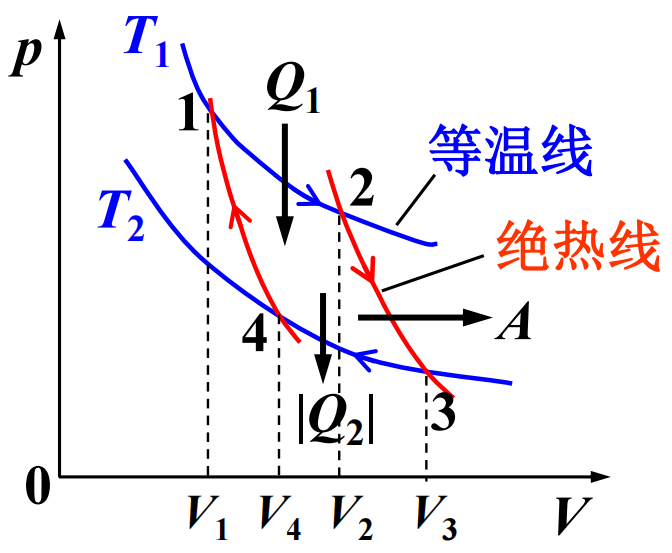
\includegraphics[width=5cm]{卡诺循环.png}
	\caption{卡诺循环示意图}
	\label{Fig: Carnot Cycle}
\end{figure}

Carnot 循环是理论上的最高效率循环,下面以理想气体为工质推导卡诺循环的效率。
\begin{itemize}
	\item 1 \(\to\) 2:等温膨胀,\(Q_1 = A_1 = \nu RT_1 \ln \dfrac{V_2}{V_1}\);
	\item 2 \(\to\) 3:绝热膨胀,\(T_1 V_2^{\gamma-1} = T_2 V_3^{\gamma-1}\);
	\item 3 \(\to\) 4:等温压缩,\(|Q_2| = |A_2| = \nu RT_2 \ln \dfrac{V_3}{V_4}\);
	\item 4 \(\to\) 1:绝热压缩,\(T_2 V_4^{\gamma-1} = T_1 V_1^{\gamma-1}\)。
\end{itemize}




\newpage
%----------------------------------------------------------
\appendix
\section{必要的数学准备}

\subsection{矢量运算}

\subsubsection{矢量乘法}

\de[矢量的标量积(点乘)]{
	两个矢量的\tboba{标量积}~$\v{A} \cdot \v{B}$是一个标量,定义为$\v{A} \cdot \v{B} := AB\cos \theta$,其中$0 \le \theta \le \upi$为$\v{A}$与$\v{B}$的夹角。
}
点乘满足交换律,因其不封闭而不满足结合律,对矢量的线性运算满足分配律。

\de[矢量的矢量积(叉乘)]{
	两个矢量的\tboba{矢量积}~$\v{A} \cp \v{B}$是一个矢量,大小定义为$\left| \v{A} \cp \v{B} \right|= AB\sin \theta$,其中$0 \le \theta \le \upi$为$\v{A}$与$\v{B}$的夹角;方向根据右手定则确定。
}
叉乘不满足交换律($\v{A} \cp \v{B} = -\v{B} \cp \v{A}$),对矢量的线性运算满足分配律。显然,对任意矢量$\v{A}$,$\v{A} \cp \v{A} = \v{0}$,于是我们规定$\v{A}^2=\v{A} \cdot \v{A}$,即$\v{A} ^2 = A^2$。

\di[矢量乘法的坐标表示]{
	在三维笛卡尔坐标系下,设两个矢量$\v{A}=\begin{bmatrix}
		A_x \\ A_y \\ A_z
	\end{bmatrix},\v{B}=\begin{bmatrix}
		B_x \\ B_y \\ B_z
	\end{bmatrix}$(或记作$\v{A}=A_x\ux + A_y\uy + A_z\uz,\v{B}=B_x\ux + B_y\uy + B_z\uz$),则
	
	(1)$\v{A} \cdot \v{B} = A_xB_x + A_yB_y + A_zB_z$;

	(2)$\v{A} \cp \v{B} = \begin{vmatrix}
		\ux & \uy & \uz \\
		A_x & A_y & A_z \\
		B_x & B_y & B_z
	\end{vmatrix} = (A_yB_z-A_zB_y)\ux + (A_zB_x-A_xB_z)\uy + (A_xB_y-A_yb_x)\uz$。
}

\di[矢量乘法的重要公式]{
	(1)$\v{A} \cdot (\v{B} \cp \v{C}) = \v{B} \cdot (\v{C} \cp \v{A}) = \v{C} \cdot (\v{A} \cp \v{B})$;

	(2)$\v{A} \cp (\v{B} \cp \v{C}) = (\v{A} \cdot \v{C}) \v{B} - (\v{A} \cdot \v{B}) \v{C}$。
}

其中,定理~\ref{矢量乘法的重要公式}(1)式具有明确的几何意义:$\left|\v{A} \cdot (\v{B} \cp \v{C})\right|$是以$\v{A},\v{B},\v{C}$为三邻边的平行六面体的体积,当$\v{A}$在$\v{B},\v{C}$按右手定则确定的一侧时可去绝对值。

\subsubsection{矢量微分}

参考实数上的定义,可以定义矢量对标量的导数。
\de[矢量对标量的导数]{
	设$\v{f}:(a,b)\rightarrow \R^n$为函数,$x_0\in (a,b)$,若
	$$\lim\limits_{x\rightarrow x_0}\frac{\v{f}(x)-\v{f}(x_0)}{x-x_0}=\lim\limits_{h\rightarrow 0}\frac{\v{f}(x_0+h)-\v{f}(x_0)}{h}$$
	存在、确定、有限,则称$\v{f}$在$x_0$处\tboba{可导},上述极限被称为函数$\v{f}$在$x_0$处的\tboba{导数},记作$\eval{\dfrac{\dif \v{f}}{\dif x}}_{x_0}$、$\mathrm{D}_x\v{f}(x_0)$等。
}

\di[矢量求导的运算法则]{
	(1)加法法则:$\dt[(\v{A}+\v{B})] = \dt[\v{A}] + \dt[\v{B}]$;

	(2)乘法法则:$\dt[(\v{A} \cdot \v{B})] = \dt[\v{A}] \cdot \v{B} + \v{A} \cdot \dt[\v{B}]$,$\dt[(\v{A} \cp \v{B})] = \dt[\v{A}] \cp \v{B} + \v{A} \cp \dt[\v{B}]$。
}

%----------------------------------------------------------
\end{document}